\documentclass{article}

%usepackages
\usepackage[utf8]{inputenc}
\usepackage{graphicx}
\usepackage[normalem]{ulem}
\usepackage{enumitem}
\usepackage{amsmath}
\usepackage[english]{babel}
\usepackage{amssymb}
\usepackage{amsthm}
\usepackage{todonotes}
\usepackage{hyperref}
\usepackage{pgf,tikz,pgfplots}
\usetikzlibrary{calc, backgrounds, positioning, fit}
\usepackage{mathrsfs}
\usepackage{dirtytalk}
\usepackage[english]{babel}
\usepackage[letterpaper, portrait, margin=1.2in]{geometry}
%\usepackage{fancyhdr}

%new commands
\newcommand{\R}{\mathbb{R}}
\newcommand{\N}{\mathbb{N}}
\newcommand{\Q}{\mathbb{Q}}
\newcommand{\Z}{\mathbb{Z}}
\newcommand{\C}{\mathbb{C}}
\newcommand{\inv}{^{-1}}
\newcommand{\img}{\textmd{Im}\:}
\newcommand{\cok}{\textmd{coker}}
\newcommand{\conv}{\textmd{conv}}
\newcommand{\vertices}{\textmd{vert}}
\newcommand{\st}{\textmd{ s.t. }}
\newcommand{\fracfield}{\textmd{frac}\:}

\newcommand{\celia}[1]{{\color{orange}[[\textbf{Celia says: }#1]]}}
\newcommand{\ad}[1]{{\color{purple}[[\textbf{Ad\'{e}lie: }#1]]}}
\newcommand{\ste}[1]{{\color{green}[[\textbf{Stefania: }#1]]}}

%new theorem environments
%plain
\theoremstyle{plain}
\newtheorem{thm}{Theorem}[section]
\newtheorem{lemma}[thm]{Lemma}
\newtheorem{prop}[thm]{Proposition}
\newtheorem*{ER}{Elder Rule}
%definitions
\theoremstyle{definition}
\newtheorem{definition}[thm]{Definition}
\newtheorem{example}[thm]{Example}
%remarks
\theoremstyle{remark}
\newtheorem{remark}[thm]{Remark}

%pgfplotsset
\pgfplotsset{compat=1.16}

%title
\title{Topology applied in Deep Learning}
\author{Luca Bracone}
\begin{document}
	\maketitle
	\tableofcontents
	\newpage
	\todo{abstract here}
	


	
\section{Basic Deep Learning}
\subsection{Neural Networks}
\begin{definition}[Perceptron]
	A \emph{Perceptron} is a function $ p:\R^n \to \R $ given by
	\[ p(x_1, \dots , x_n) = g \left( w_0 + \sum_{i=1}^{n} w_i x_i \right)\]
	\begin{center}
	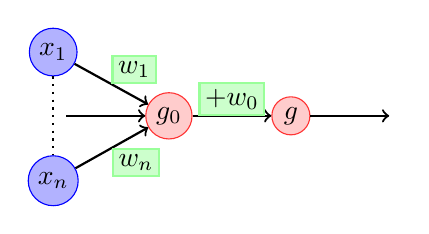
\begin{tikzpicture}[inner sep= 2pt]
	\node (x1) [circle, draw= blue, fill= blue!30] at (0,0) {$x_1$};
	\node (xn) [circle, draw= blue, fill= blue!30] [below= of x1] {$x_n$};
	\path[thick, dotted] (x1) edge node[name=dots,right]{} (xn);
	\node (g0) [right= of dots,circle, draw=red!80, fill= red!20] {$g_0$};
	\path[thick, ->] (x1) edge node[auto, rectangle, draw=green!40, fill=green!20]{$w_1$} (g0)
	                 (dots) edge (g0)
	                 (xn) edge node[auto,swap, draw= green!40, fill= green!20]{$w_n$} (g0);
	\node (g) [right= of g0, circle, draw=red!80, fill=red!20] {$g$};
	\path[thick, ->] (g0) edge node[auto, draw= green!40, fill=green!20] {$+w_0$} (g);
	\node (out) [right= of g] {};
	\path[thick, ->] (g) edge (out);
	\end{tikzpicture}
	\end{center}
	Where $ w_1, \dots, w_n \in \R $ are called the \emph{weights} of $p$, $w_0$ is called the \emph{bias}, and $g:\R \to \R $ is any non-linear function called the \emph{activation function}.
	Most of the time we use as activation function \[ g(x)=\frac{e^x}{e^x+1}, \] the sigmoid function.
	\end{definition}

\begin{definition}[Artificial Neural Network]
	A (forward-feeding) \emph{Artificial Neural Network} (ANN) is a function $T: \R^n \to \R^m$ that can be decomposed as  \[ T= l_k \circ \dots \circ l_1 ,\] where the $l_i : \R^{n_i} \to \R^{n_{i+1}}$ are called \emph{layers} and are just vectors of perceptrons \[ l_i(\vec{x})=(p_{i,1}(\vec{x}),\dots,p_{i,n_{i+1}}(\vec{x})). \] The first layer $l_1$ is also called input layer, the others are called hidden layers.
	In the context of neural networks perceptrons are also called nodes.
	\begin{figure}[h]
	\centering
	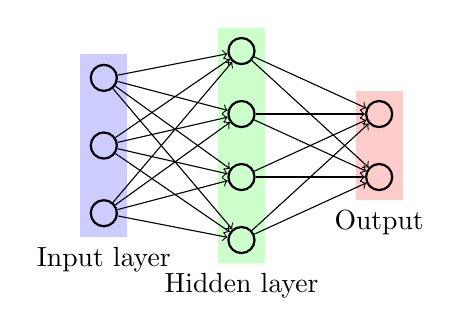
\begin{tikzpicture}[vertex/.style={draw=black,thick, circle}, node distance = .5cm]
		\node (x1) [vertex] {};
		\node (x2) [vertex, below= of x1] {};
		\node (x3) [vertex, below= of x2] {};
		\node (layer1 center) at ($1/3*(x1)+1/3*(x2)+1/3*(x3)$) {};
		\node (layer2 center) [right=1.5cm of layer1 center] {};
		\node (g1) [vertex] at ($(layer2 center) + (0,1.5*.8cm)$) {};
		\node (g2) [vertex] at ($(layer2 center) + (0,.5*.8cm)$) {};
		\node (g3) [vertex] at ($(layer2 center) + (0,-.5*.8cm)$) {};
		\node (g4) [vertex] at ($(layer2 center) + (0,-1.5*.8cm)$) {};
		\node (layer3 center) [right=1.5cm of layer2 center] {};
		\node (y1) [vertex] at ($(layer3 center) + (0,.5*.8cm)$) {};
		\node (y2) [vertex] at ($(layer3 center) + (0,-.5*.8cm)$) {};
		\foreach \n in {1,2,3}
		    \foreach \m in {1,...,4}
		        \path[->] (x\n) edge (g\m);
	    \foreach \n in {1,...,4}
	        \foreach \m in {1,2}
	            \path[->] (g\n) edge (y\m);
	    \begin{scope}[on background layer]
	    \node (input layer) [rectangle, fit=(x1)(x2)(x3), fill= blue!20, label=below:Input layer] {};
	    \node (hidden layer) [rectangle, fit=(g1)(g2)(g3)(g4), fill=green!20, label=below:Hidden layer] {};
	    \node (output) [rectangle, fit=(y1)(y2), fill=red!20, label=below:Output] {};
	    \end{scope}
		\end{tikzpicture}
		\label{fig:neural-network}
		\caption{An example neural network with three input nodes, one hidden layer, and two output nodes}
		\end{figure}
		\todo{in this picture, put arbitrarily many hidden layers}
	\end{definition}
%\end{minipage}
For some ANN, $T$ and some input $ (x_1,...,x_n) $, we denote $ (y_1,...,y_n) $ the desired output of $ T $. We denote also $ (\hat{y}_1,...,\hat{y}_m) $ the output $T$ actually produced.
\begin{definition}[Loss Function]
	 The \emph{loss} ( sometimes called \emph{cost})  associated to a neural network $T$ for a given input is a function that measures the `` distance" between the produced and desired output of the network. For most basic applications, the loss is defined as the $l^2$ norm on $\R^n$
	\[\mathcal{L}(W; x)= \sum_{i=1}^{m} ||y_i - \hat{y}_i||_2^2 , \]
	where $W$ is the set of all the weights and biases of every perceptron in $T$.
\end{definition}
\begin{definition}[Empirical Loss]
	For a set of inputs $X=\{(x_1^1,\dots,x_n^1), \dots , (x_1^m,\dots ,x_n^m)\}$, and $T$ an ANN, the \emph{Empirical Loss} is defined as
	\[ J(W)=\frac{1}{|X|} \sum_{\vec{x}\in X} \mathcal{L}(W;x), \]
	the average loss over $X$.
\end{definition}
\begin{example}
Suppose we are some school's administrative staff and we would like to predict whether or not a given student is going to pass a certain class by using a neural network. This neural network would output a number $\hat y$ between $0$ and $1$ reflecting how likely it is that he or she is going to pass. We may feed as inputs as many parameters as we would like, but for now let us limit ourselves to two: $x_1$ represents how many hours per week this student works on this class, and $x_2$ could be the overall talent of this student. We might decide to use the following neural network:
\begin{center}
    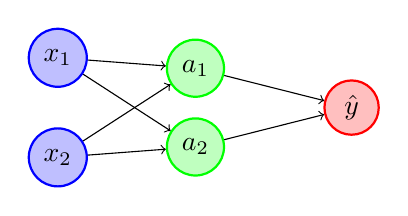
\begin{tikzpicture}[
    input/.style=
    {draw=blue, fill=blue!25, thick, circle}, midput/.style=
    {draw=green, fill= green!25, thick ,circle},
    node distance = .5cm]
    \node (x1) [input] {$x_1$};
    \node (x2) [input, below= of x1] {$x_2$};
    \node (layer1 center) at ($1/2*(x1)+1/2*(x2)$) {};
    \node (layer2 center) [right=1.5cm of layer1 center] {};
    \node (a1) [midput] at ($(0,.5cm) + (layer2 center)$) {$a_1$};
    \node (a2) [midput] at ($(0,-.5cm) + (layer2 center)$) {$a_2$};
    \node (y) [draw=red, fill=red!25, circle, thick, right=1.5cm of layer2 center] {$\hat y$};
    \foreach \n in {1,2}
        \foreach \m in {1,2}
            \path[->] (x\n) edge (a\m);
    \path[->] (a1) edge (y) (a2) edge (y);
    \end{tikzpicture}
\end{center}
We choose to only add a single hidden layers of two nodes because the conditions of the problem are relatively simple. Although we are free to experiment with more input parameters or additional and bigger hidden layers, it is better to restrain ourselves in that regard for reasons we shall explain in section~\ref{subsection:overfitting} Unfortunately, no matter how we try to shape the neural network, the output seems to be randomly generated. In fact, it is random. The reason for that is that we have not calibrated the weights (not drawn in the picture above, but always present) of the neural network to obtain a reliable output. In the next section, we will see how to make use of the loss function to make efficient changes to the weights.
\end{example}

\subsection{Gradient Descent}
%The output of a neural network depends on the weights and biases of its perceptrons. In order to have the output of the neural network as close as possible to the desired output, one has to find an efficient way to tweak the weights such that the empirical loss becomes as low as possible. To accomplish this task we make repeated use of an algorithm called gradient descent.
%Applying this algorithm involves taking a step in the direction for which the empirical loss is minimised until we reach a stopping condition.  For each weight $w_i$ in $T$, we denote the vector $ \left(\frac{\partial J}{\partial w_i} \right)_{i\in I} $ as $\nabla J$, where $ \frac{\partial J}{\partial w_i} $ with $w_i$ being any weight in $T$, represents how big of a change in $J$ we will obtain by moving $w_i$. The gist of the algorithm revolves around updating the weights with the rule $W \gets W - \eta \nabla J$. Where $\eta$ is a constant that has to be well chosen. If this constant is too small, gradient descent would stop when it meets the slightest uphill. Thus it would miss a better minimum which might be close by. If the constant $\eta$ is too big, gradient descent can only take giant steps and it would diverge to infinity.
By now, we have understood that what really determines the output of a neural network are its weights and biases. Suppose we are given a set of inputs $X \subset \R^n$ each of which is labeled with its desired output. For example, if $X$ is a set of hand drawn images of digits, the label tells us what digit it's supposed to be. The task of the neural network would be to tell what digit each image represents (In general, it would be for $T(x)$ to be as close to its label as possible). Let's imagine this network $T$ to be comprised of one input for each pixel in the image (each pixel being a real number in $[0,1]$), a certain number of hidden layers, and $10$ output nodes (reflecting how likely the networks thinks that this image is a certain digit). Let's test the network with the image of a three. At the beginning its guess is as good as random and we calculate a relatively big loss $J(W)$. Fortunately we know that $T$ is differentiable, so for each weight we can calculate its gradient $\partial J / \partial w_i$ which is a number that tells us how big of a change (positive of negative) in $J$ we are going to obtain by moving $w_i$. The vector $(\partial J / \partial w_i)_{i\in I}$ is written $\nabla J$ and tells us the fastest direction to increase $J$ for a certain set of inputs $X$. We want $J$ to be as low as possible so we will take a small step in the opposite direction: \[W_{new}= W_{old} - \eta \nabla J, \] where $\eta$ is a constant that's picked to be not too small or too big. By repeatedly applying this algorithm, we obtain a set of weights $W$ that minimizes $J(W)$. This minimum is only local, and restarting this process with new random weights is going to produce new minimizing weights. Applying this algorithm repeatedly is called \emph{training}.\\	In practice, computing the derivative with respect to some particular weights is not difficult. Consider the following neural network: \\
		\begin{center}
        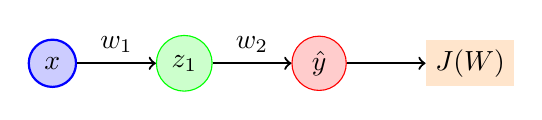
\begin{tikzpicture}[perceptron/.style={circle, draw=blue,fill=blue!20,thick, inner sep=0mm, minimum size= 6mm},
        scalar/.style={rectangle, fill=orange!20}]
        \node (input) [perceptron] {$x$};
        \node (hidden) [circle, draw= green, fill= green!20, right= of input] {$z_1$}; 
        \node (output) [circle, draw= red, fill=red!20 , right= of hidden] {$\hat{y}$};
        \node (loss) [scalar, right = of output] {$J(W)$};
        \draw[->, thick] (input) to node[auto] {$w_1$} (hidden);
        \draw[->, thick] (hidden) to node[above] {$w_2$} (output);
        \draw[->, thick] (output) to (loss);
		\end{tikzpicture}
		\end{center}
The gradient descent can be computed with an application of the chain rule:\[
\frac{\partial J}{\partial w_2} =\frac{\partial J}{\partial \hat{y}} \frac{\partial \hat{y}}{\partial w_2} \qquad
\frac{\partial J}{\partial w_1} = \frac{\partial J}{\partial \hat{y}}\frac{\partial \hat{y}}{\partial z_1}\frac{\partial z_1}{\partial w_1} \]

\noindent \textbf{Data batching:} Since calculating $\nabla J$ is computationally intensive, one may be intersting in \emph{batching} the dataset. That is, taking a random subset of the data and applying gradient descent to it instead. The convergence is going to be more erratic, depending on the size of the subset chosen.
\subsection{Overfitting}\label{subsection:overfitting}
%When training our neural network, it might happen that it essentially \say{learns the data set by heart} making it unable to properly tackle on never seen before data points. There are a few methods to avoid such a problem:
Now comes the question of when should we stop the training. For that we reserve a subset of the data on which we never apply gradient descent. Effectively, this makes the network never be able to learn from it. For that reason we call it testing set, as opposed to the training set. We then decide to stop the training if the network consistently starts performing worse on the testing set, than it did previously. 
	\begin{figure}[h]
	\centering
	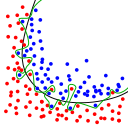
\includegraphics{overfitting.png}
	\caption{An over-fitted neural network \protect \footnotemark}
	\label{fig:overfitting}
	\end{figure}
	\footnotetext{Courtesy of wikimedia foundation \href{https://commons.wikimedia.org/wiki/File:Overfitting.svg}{https://commons.wikimedia.org/wiki/File:Overfitting.svg}}
	
What happens if we train the network more than that? Then, we might reach a situation like the one illustrated in figure~\ref{fig:overfitting}. This network was tasked with finding a line between the blue and red dots. We can imagine the situation where the dots are the result of some experiment, the separation being in the shape of a parabola a theoretical prediction. The dots that seem to have leaped over could be explained as being caused by small errors produced by the measuring equipment. Because we have over-trained our neural network, it is missing the bigger picture and focusing excessively on the training data. Therefore When presented with new data the network is prone to more errors than if we had trained it less.

Overfitting may also arise in the same way if we choose too many input parameters or if we have too deep or wide hidden layers, or additionally if by bad luck the network comes to focus too much on one specific node. For the last case to not happen we can apply \emph{dropout} during training. That is, to randomly set some (typically half) of the nodes to output zero no matter what inputs are fed by the previous layer. This makes the network more robust when presented with previously unseen data.
%\emph{Dropout} involves randomly setting some nodes to zero during training. This makes the network not rely too much on some path.
%\emph{early stopping} is the process by which after each application of gradient descent, one tests the network. If it performs worse than it did previously, stop the training process.	

\section{Simplicial Complexes}
\begin{definition}[Convex Hull]
Let $ u_0,...,u_k \in \R^n $ their \emph{convex hull} is defined as
\begin{equation} 
\label{conv-hull}
\conv \{u_0,...,u_k\} = \left\{ x= \sum_{i=0}^{n} \lambda_i u_i \ :    \sum_{i=0}^{n} \lambda_i = 1; \ \lambda_i > 0 \ \forall i \right\} 
\end{equation}
\end{definition}
	
Let $u_0,...,u_k \in \R^n$ . They are said to be \emph{affinely independent }if for any point in their convex hull the coefficients $\lambda_i$ are unique.	

\begin{definition}[$k$-simplex]
A \emph{$k$-simplex} is the convex hull of $k$ affinely idependent point. 
\end{definition}
The \emph{dimension} of a $k$-simplex is $k$.
\begin{definition} [Faces and Co-faces]
Let $ \{u_{i_0},...,u_{i_m} \}$ be a subset of $\{u_0,...,u_k\} $. In this case, we say that $ \tau = \conv\{u_{i_1},...,u_{i_m}\} $ is a \emph{face} of $ \sigma = \conv\{u_1,..,u_k\} $ which we write $ \tau < \sigma $. Equivalently, $ \sigma $ is said to be a \emph{co-face} of $ \tau $.
\end{definition}
	
\begin{definition}[Simplicial Complex]
A \emph{simplicial complex} $K$ is a collection of simplices such that:
\begin{enumerate}[label=(S\arabic*)]
	\item $ \forall \sigma \in K, \ \tau < \sigma \implies \tau \in K $. 
	\item $ \forall \sigma,\tau \in K, \ \sigma \cap \tau $ is either empty or a face.
\end{enumerate}
The \emph{dimension} of the simplicial complex $K$ is defined as $ \dim K = \max_{\sigma \in K} \dim \sigma $.
	The \emph{underlying space} of $K$, denoted by $|K|$ is the topological space $ \bigcup_{\sigma \in K} \sigma $ with the subspace topology.
	\end{definition}
\todo{simple examples of complexes}
\begin{definition}[Triangulation]
	Let $X$ be a topological space and $K$ a simplicial complex, if there exists a homeomorphism $ \phi : X \to |K| $ we say that $X$ is triangulable. In that case the couple $ (K,\phi) $ is called a triangulation of $X$
\end{definition}

	\begin{definition}[Sub-complex]
		A subset $L \subseteq K$ is a \emph{sub-complex} of K if it is itself a simplicial complex. It is called full if it contains all vertices of $K$.
	\end{definition}
	
	\begin{definition}[Skeleton]
		The \emph{$j$-skeleton} of a simplicial complex $K$ is the subset of simplices $K^{(j)}= \{ \sigma \in K \st \dim\sigma \leq j \} \subseteq K $. In particular the 0-skeleton is denoted by $\vertices(K)$ and it consists of the vertices of $K$
	\end{definition}
	
	\begin{definition}[Star and Link]
		Let $K$ be a simplicial complex and pick $ \sigma \in K $. Its \emph{star}, is the set \[ st (\sigma) = \{ \tau \in K \st \tau < \sigma \} \].\ste{point shoulg go in previous line}
		Let $\overline{st} (\sigma)$ be the smallest sub-complex that contains $st(\sigma)$, we call it the \emph{closed star} of $\sigma$. \\
		Similarly, the \emph{link} of a simplex \[ lk (\sigma) = \{ \tau \in \overline{st}(\sigma) \st \tau \cap \sigma = \emptyset \} \] the set of simplices in the closed star that do not touch \ste{attention to abbreviation. Check this in the text}$\sigma$.
	\end{definition}
	\begin{remark}
        Note that the star of a $k$-simplex $\sigma$ is not necessarily a sub-complex of $K$ because it is not closed under taking faces. This motivates the definition for the closed star $ \overline{st} (\sigma) $.
	\end{remark}
	\begin{definition}[Simplicial Maps and Homeomorphisms]
		Let $K$, $L$ be two simplicial complexes and $ \phi: \vertices ( K) \to \vertices (L) $ a map such that vertices of every simplex in $K$ gets mapped to a vertex of a simplex in $L$, in that case $\phi$ is called a \emph{vertex map}. The map $f: |K| \to |L|$ defined by $ \sum_{i=0}^n \lambda_i u_i \mapsto \sum_{i=0}^n \lambda_i \phi(u_i) $ is called a \emph{simplicial map}. If $ \phi $ is bijective and $ \phi\inv $ is also a vertex map, we call it instead a \emph{simplicial homeomorphism}.
	\end{definition}

	\section{Simplicial Homology}
	\begin{definition}[$p$-chain]
		Let $K$ be a simplicial complex. A \emph{$ p $-chains} is a formal sum of its $p$-simplices of $K$ over a field $F$ \[ c = \sum_{i=1}^{n} a_i \sigma_i. \] Where $\sigma_i \in K$ and $a_i \in F$.
	\end{definition}
	For the time being, the field in question is $F = \mathbb{F}_2 $. Component-wise addition of chains $ c + d = \sum_{i=1}^n (c_i + d_i) \sigma_i $ makes the set of $p$-chains into a commutative group which we note as $ (C_p, +) $.
\begin{definition}[Boundary]
	The \emph{boundary} is a map $ \partial_p : C_p \to C_{p-1} $ which for a $p$-simplex returns the sum of the $ (p-1) $-faces: \[ \partial_p \sigma = \sum_{j=1}^n [u_1, \dots , \hat{u}_j , \dots , u_p] \]
	where $[ u_1 \dots u_p ]$ is the $p$-simplex given by the convex hull of $\{u_1, \dots , u_p\}$ and $\hat{u}_j$ means we omit the $j$-th term from that notation.
	This definition extends by linearity to the $p$-chains: \[ \partial_p c = \sum_{i=1}^{n} a_i \ \partial_p\sigma_i  \]
\end{definition}
It turns out that $ \partial_p : C_p \to C_{p-1} $ is a group homomorphism. For a simplicial complex $K$ we define its chain complex as
\[\mathcal{C}_K: \ \dots \longrightarrow C_p \stackrel{\partial_p}{\longrightarrow} C_{p-1} \stackrel{\partial_{p-1}}{\longrightarrow} \dots \stackrel{\partial_1}{\longrightarrow} C_0 \longrightarrow 0 \]

\begin{thm}[Fundamental Lemma of Homology]For all $p$ and $d \in C_{p+1}$, we have $ \partial_{p} \partial_{p+1} d = 0$
\end{thm}

Whenever we have an interesting homomorphism it is natural to want to know more about its kernel and image, in this case they have special names.

\begin{definition}[$p$-boundaries and $p$-cycles]
	The \emph{$p$-cycles} are the elements which belong to the kernel of the boundary \[Z_p:= \ker\partial_{p} = \{ c \in C_p : \partial_p c = 0 \} \]
	The \emph{$p$-boundaries} are the elements which are given as the boundary of a $(p+1)$-chain \[B_P := \img\partial_{p+1} = \{ c \in C_p : \exists d \in C_{p+1} , \ c=\partial_{p+1} d \} \]
\end{definition}

\begin{remark}
Whenever it is clear, we favour the notation $\partial$ over $\partial_p$, omitting the $p$. 
\end{remark}
\begin{remark}
Furthermore, note that if $ c \in B_p $ then $ \partial c = \partial \partial d = 0 $. Thus, we notice that $ B_p \subseteq Z_p $. But in general $ B_p \neq Z_p $. %In particular, we are interested in the $p$-cycles that are not $p$-boundaries.
The difference between $p$-cycles and $p$-boundaries is what motivates the definition of homology groups.
\end{remark}

\begin{definition}[Homology Groups and Betti numbers]
	For a complex $K$ its $p$-th \emph{homology group} is the quotient  \[H_p = Z_p/B_p \].\\
	The $p$-th \emph{Betti number} is $ \beta_p $ the number of generators of $H_p$.
\end{definition} 

\begin{figure}[h!]
\begin{center}
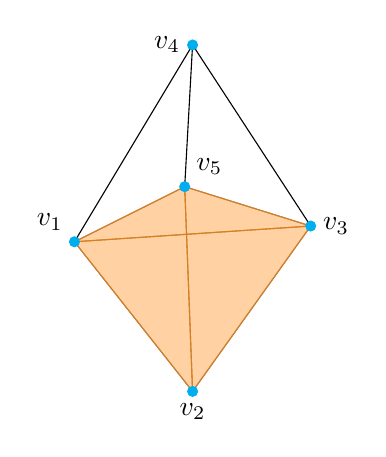
\begin{tikzpicture}[node distance = 1pt]

\coordinate (v2) at (0,-3.5) {};
\node[below= of v2] {$v_2$};
\coordinate (v1) at (-1.5,-1.6) {};
\node[above left= of v1] {$v_1$};
\coordinate (v3) at (1.5,-1.4) {};
\node[right= of v3] {$v_3$};
\coordinate (v4) at (0,0.9) {};
\node[left= of v4] {$v_4$};
\coordinate (v5) at (-0.1,-0.9) {};
\node[above right= of v5] {$v_5$};

\draw[brown] (v1) -- (v2) -- (v3) -- cycle;
\draw[brown] (v5) -- (v2) -- (v3) -- cycle;
\draw[brown] (v1) -- (v5) -- (v3) -- cycle;
\draw[brown] (v1) -- (v2) -- (v5) -- cycle;

\fill[orange, opacity=0.2] (v1) -- (v2) -- (v3) -- cycle;
\fill[orange, opacity=0.2] (v5) -- (v2) -- (v3) -- cycle;
\fill[orange, opacity=0.2] (v1) -- (v5) -- (v3) -- cycle;
\fill[orange, opacity=0.2] (v1) -- (v2) -- (v5) -- cycle;
\draw (v1) -- (v4) -- (v3);
\draw (v4) -- (v5);
\foreach \n in {1,...,5}
    \fill[cyan] (v\n) circle (2pt);
\end{tikzpicture}
\caption{An example of a simplicial complex embedded in $\R^3$}
\label{fig:example1}
\end{center}
\end{figure}

\begin{example}
Consider the simplicial complex in figure~\ref{fig:example1}. It consists of the union of two tetrahedrons except that for the upper one we removed its volume as well as all its faces, while for the bottom one we remove its volume \ste{One can rephrase this by saying that it is the union of the 1-skeleton and 2-skelton of a tetrahera.}.
We will now compute its homology groups. \\ First notice that $H_0 = \langle [v] \rangle $ where $[v]$ is the equivalence class of any $0$-chain whose sum is comprised of a single vertex. Indeed, for $\partial: C_0 \to 0$ the kernel is the whole group $C_0$. On the other hand, since $K$ has one connected component, for any two vertices $u,w$ there is a $1$-chain, which can be thought of as a path between $u$ and $w$, such that its boundary is $u+w$. Thus, $B_0$ is comprised of the $0$-chains that have an even number of summands. Therefore $H_0$ contains only one non-trivial class, namely the $0$-chains that are the sum of an odd number of vertices which are equivalent to the $0$-chains with only one summand. The choice of $v$ for the representative does not matter because $K$ has one connected component. For every vertex $x,y$ we can write 
\[v = v+0 = v + \partial p_{x,y} = v + x + y = \partial p_{v,x} + y = y.  \] Where $p_{x,y}$ denotes a $1$-chain whose boundary is $x+y$. \\
Now for $H_1$, to alleviate the notation we write $e_{i,j}$ for the $1$-simplex $(v_iv_j)$. We notice that there are three 1-chains that form a face of three  “empty triangles”. Namely, the $1$-chains \[f= e_{1,4} + e_{4,3} + e_{3,1},\ g=\ e_{5,4} + e_{4,3} + e_{3,5} \text{ and } h=\ e_{1,4} + e_{4,5} + e_{5,1} \ste{I took out =\ e_{1,5} + e_{5,3} + e_{3,1}, I think this is not a face of an empty triangle}\] are cycles, but that they are not the boundary of any 2-chain. Thus for each empty face, we have a generator of $H_1$. There are no other generators because for any other $1$-cycle we may sum it with a certain combination of the following $1$-chains \[ e_{1,2} + e_{2,3} + e_{3,1}, e_{5,2} + e_{2,3} + e_{3,5}, e_{1,5} + e_{5,3} + e_{3,1}, e_{1,2} + e_{2,5} + e_{5,1} \]  in order to find one that we have already found. \ste{We can discuss the lines above during our next meeting.} For example
\[ e_{1,2} + e_{2,3} + e_{3,4} + e_{4,1} \ + \ e_{1,2} + e_{2,3} + e_{3,1} = e_{1,4} + e_{4,3} + e_{3,1} .\] So, $H_1$ is the free commutative group generated by $\{f,g,h\}$ where $f,g,h$ are the 1-chains that each correspond to one of the empty triangles in the upper tetrahedron. \\
Lastly, for $H_2$ there is only one 2-cycle that is not a 2-boundary This is the “shell” of the bottom tetrahedron which by construction is empty. Therefore, $H_2$ is the free group generated by the 2-chain that corresponds to that shell \ste{Perhaps writing what is the shell}. If that volume were to be full, $H_2$ would instead be trivial.\\
The group $H_3$ is trivial because there are no 3-chains. \\
We see that the Betti numbers are $\beta_0 = 1$, $\beta_1 = 3$, $\beta_2 = 1$, $\beta_n = 0$ for all $n \geq 3$
In general, $\beta_0$ can be thought of as the number of connected components, $\beta_1$ as the number of holes, $\beta_2$ the number of empty volumes, and  $\beta_n$ as the number of \say{$n$-dimensional holes}.
\end{example}


\begin{definition}[Induced Map]
	Consider two complexes $K$, $L$ and a simplicial map $ f: K \to L $. We have a way to transform $f$ into a map $ f_\sharp: C_p(K) \to C_p(L) $, in this way 
	\[ c = \sum_{i=1}^n a_i \sigma_i \ \mapsto \ \sum_{i=1}^n a_i \tau_i  \]
	Where $ \tau_i = f(\sigma_i) $ if it has dimension $p$ or $ \tau_i =0 $ otherwise. We call $f_\sharp$ the \emph{induced map} of $f$.
\end{definition}

\section{Persistent Homology}

\begin{definition}[Level Sets]
For a topological space $X$ and a map $f:X\to \R$, its \emph{level sets} are $ X_a=\{ x \in X \st f(x) \leq a\} $
\end{definition}

Suppose $f$ is continuous. For each $X_a$ we consider its connected components, we can imagine a picture where on the vertical axis we have the real number line and horizontally we plot a point for each connected component of $X_a$. This effectively gives a graph, and if $f$ is monotone, a tree. \ste{How are the edges of this graph constructed?} This is called the \emph{merge tree} of $X$ under $f$. Its vertices are located at times where two components merge, and the edges represent the existence of a component over time. \\
We would like to attach an identity to these components, so we use the following rule:
\begin{ER}
When two components merge, we keep the oldest one. The younger is said to die or to merge into the older one.
\end{ER}

Using the level sets, we define an increasing chain of sub-complexes. Indeed, if $f:K \to \R$ is monotone (that is whenever $\sigma < \tau$, $f(\sigma) < f(\tau)$) and continuous, the level sets $f\inv(-\infty, a] = K(a)$ are sub-complexes of $K$. \\
We now write $K_i$ instead of $K(a_i)$.
\begin{definition}[Filtration]
Let $K$ be a complex. The sequence of inclusions,
\[ \emptyset = K_0 \subseteq K_1 \subseteq \dots \subseteq K_{n-1} \subseteq K_n = K \] is called a \emph{filtration} of $f$.
\end{definition}

From a filtration we obtain a sequence of homology groups 
\[ H_p(K_0) \rightarrow \dots \rightarrow H_p(K_n) \] where the arrows are the homomorphisms induced by the inclusion maps.

\begin{definition}[Persistent Homology Groups and Persistent Betti Numbers]
Considering the above chain of homology groups, the $p$-th persistent homology groups are defined as $H_p^{i,j} := \img f_p^{i,j}$. Where $f_p^{i,j}: H_p(K_i) \hookrightarrow H_p(K_j)$ is the homomorphism induced by the inclusion. \\
The $p$-th persistent \emph{Betti Number}, $\beta_p^{i,j}$ is the number of generators of $H_p^{i,j}$
\end{definition}
\begin{remark}
Under this definition, $H_p^{i,i}$ is the $p$-th homology group of $K_i$
\end{remark}
\newpage %this is needed only if "example" and the tikz image keep showing on different pages
\begin{example}\ \\
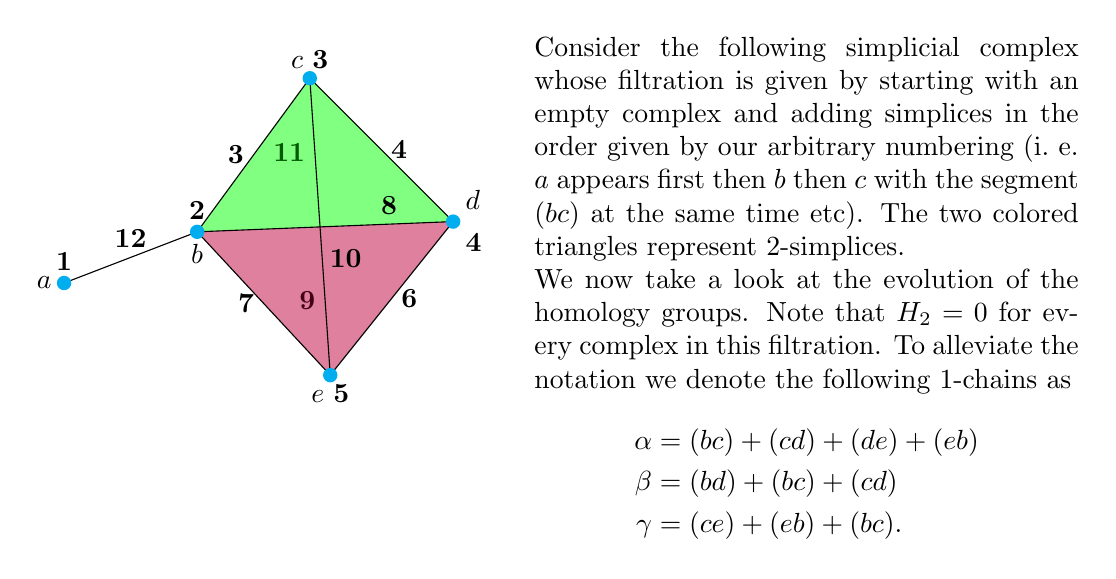
\begin{tikzpicture}[scale=1.3]

\coordinate (a) at (0.5,0.5);
\node[left=1pt of a] {$a$};
\node[above=1pt of a] {\textbf{1}};
\coordinate (b) at (1.8,1);
\node[below=1pt of b] {$b$};
\node[above=1pt of b] {\textbf{2}};
\coordinate[label=above:{$c$ \textbf{3}}] (c) at (2.9,2.5);
\coordinate (d) at (4.3,1.1) ;
\node[above right=.5mm of d] {$d$};
\node[below right=.5mm of d] {\textbf{4}};
\coordinate[label=below:{$e$ \textbf{5}}] (e) at (3.1,-0.4);

\fill[color=green!50] (b) -- (c) -- (d) -- cycle;
\fill[color=purple!50] (b) -- (d) -- (e) -- cycle;

\draw (a) -- node[above] {\textbf{12}} (b) -- node[left] {\textbf{3}} (c) -- node[right] {\textbf{4}}  (d) -- node[right]{\textbf{6}} (e) -- node[left] {\textbf{7}} (b) -- node[auto, near end] {\textbf{8}} (d);
\draw (c) -- node[left, near start, color=black!65!green] {\textbf{11}} node[left, near end, color=black!65!purple](eleven) {\textbf{9}} node[below=.4cm of eleven, right] {\textbf{10}} (e);

\foreach \point in {a,b,c,d,e}
    \fill[cyan] (\point) circle (2pt);

\node [below right, text width=.57\textwidth,align=justify] at (5,3) {Consider the following simplicial complex whose filtration is given by starting with an empty complex and adding simplices in the order given by our arbitrary numbering (i.\ e. $a$ appears first then $b$ then $c$ with the segment $(bc)$ at the same time etc). The two colored triangles represent $2$-simplices. \\ We now take a look at the evolution of the homology groups. Note that $H_2=0$ for every complex in this filtration. To alleviate the notation we denote the following 1-chains as 
\begin{align*}
    \alpha &= (bc)+(cd)+(de)+(eb) \\
    \beta  &= (bd)+(bc)+(cd) \\
    \gamma &= (ce)+(eb)+(bc).
\end{align*}};
\end{tikzpicture}
\\
We calculate the following homologies:
\begin{center}
\begin{tabular}{|l|l|l|l|l|l|}
    \hline
     \textbf{(1)}&\textbf{(2)}&\textbf{(3)}&\textbf{(4)}&\textbf{(5)}&\textbf{(6)}  \\
     $ H_0=\langle a \rangle $ & 
     $ H_0=\langle a,b \rangle $ &
     $ H_0=\langle a,b \rangle $ &
     $ H_0=\langle a,b \rangle $ &
     $ H_0=\langle a,b,e \rangle $ &
     $ H_0=\langle a,b \rangle $ \\
     $H_1 = 0$ &
     $H_1 = 0$ &
     $H_1 = 0$ &
     $H_1 = 0$ &
     $H_1 = 0$ &
     $H_1 = 0$ \\
    \hline
     \textbf{(7)}&\textbf{(8)}&\textbf{(9)}&\textbf{(10)}&\textbf{(11)}&\textbf{(12)}\\
     $ H_0=\langle a,b \rangle $ &
     $ H_0=\langle a,b \rangle $ &
     $ H_0=\langle a,b \rangle $ &
     $ H_0=\langle a,b \rangle $ &
     $ H_0=\langle a,b \rangle $ &
     $ H_0=\langle a \rangle $ \\
     $H_1=\langle \alpha \rangle$ &
     $H_1=\langle \alpha,\beta  \rangle$ &
     $H_1=\langle \alpha \rangle$ &
     $H_1=\langle \alpha, \gamma \rangle$ &
     $H_1=\langle \gamma \rangle$ &
     $H_1=\langle \gamma \rangle$ \\
    \hline
\end{tabular}
\end{center}
(If the reader wants to compute the same table, we recommend he or she draws a picture for each complex in the filtration).\\
Notice how in step 12, it is $a$ that is kept, rather than $b$. This is the elder rule in action.
Notice how in step 8, we might think that two new generators were added, one for each empty triangle, but in reality only $\beta$ is added. The other one is a sum of the generators who are already present:
\[(be)+(ed)+(db)=(bc)+(cd)+(de)+(eb)+(bc)+(cd)+(bd)= \alpha + \beta  \]
Likewise in step 10 one might think that a generator is added for each of the two empty triangles created but only one is really added. The other one is a sum of the two:
\[ (ed)+(dc)+(ce) = (ce)+(eb)+(bc)+(bc)+(cd)+(de)+(eb) = \gamma + \alpha \]
\ste{Discuss the homology for parameter greater than 9 in the next meeting.}
\end{example}

The classes of $H_p(K_i)$ represent $p$-dimensional holes \say{when viewing $K$ at a certain resolution}. It is then clear that if a certain $p$-dimensional hole is visible for various resolutions, then it somehow exists or represents an important feature in the \say{real complex}. To make this idea clearer we introduce the following vocabulary.

\begin{definition}
Let $\gamma \in H_p^{i,i} $. If $\gamma \notin H_p^{i-1,i}$ we say that $\gamma$ is \emph{born at $K_i$}. \\
Furthermore if $f_p^{i,j-1}(\gamma) \notin H_p^{i-1,j-1}$ and $f_p^{i,j} \in H_p^{i-1,j}$ then we say that $\gamma$ \emph{dies entering $K_j$} \\
The \emph{persistence} of $\gamma$ is the number $a_j-a_i$
\end{definition}

Let $\mu_p^{i,j}$ be the number of classes born at $K_i$ and dying at $K_j$. In other words 
\[ \mu_p^{i,j} = \left( \beta_p^{i,j-1} - \beta_p^{i,j} \right) - \left( \beta_p^{i-1,j-1} - \beta_p^{i-1,j}  \right). \]
Indeed, the first difference counts the classes that are born at or before $K_i$ and that die entering $K_j$ while the other counts those that are born strictly before $K_i$ and die entering $K_j$.

We now look for a way to visualise all the gained information. For that, we look to \emph{Persistence Diagrams}. For each class that appears, draw a point at coordinates $(a_i,a_j)$ with multiplicity $\mu_p{i,j}$. Where $a_i$ is when it was born and $a_j$ when it died.

\begin{example}
Consider the persistence diagram illustrated in figure~\ref{fig:torus-rips-persisntence} on page~\pageref{fig:torus-rips-persisntence} computed using Vietoris-Rips filtration. It represents the persistence classes of a point cloud in the shape of a torus \ste{Maybe adding the point cloud?}. The points that stick out from the diagonal are the classes whose persistence is greater, and thus most worthy of attention. We can see that the fact there is only one connected component is quickly detected. We also see that the filtration identifies four classes of 1-dimensional holes, two disappear quickly and the other two (which are almost stacked on top of each other) are the loops on the torus we already are familiar with \ste{Maybe tell what is the homology of the toprus because we did not talk about it in this report}. Finally, the 2-dimensional hole, i.e the \say{volume} of the torus, is clearly identified \ste{Tell by which poin in the diagram, eg the purple point}.
\end{example}

\begin{figure}[ht]
    \centering
    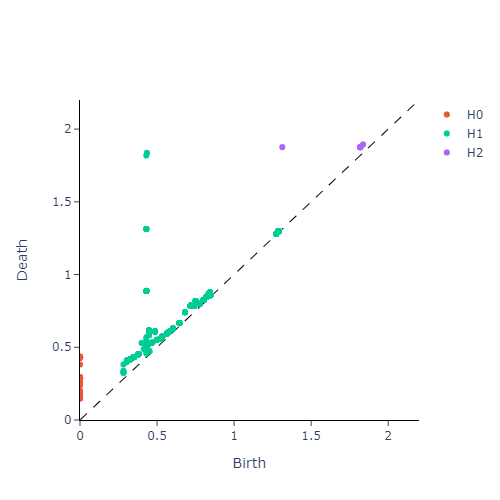
\includegraphics[scale=.5]{torus-rips-persistence.png}
    \caption{Persistence diagram of a torus}
    \label{fig:torus-rips-persisntence}
\end{figure}

\section{Cubical Homology}
\ste{I would put this section after simplicial homology. Celia and Adelie, what do you think?}
\begin{definition}[Elementary Interval]
Let $z \in \Z$ an integer. \emph{Elementary intervals} are subsets of $\R$ the form $ [z,z+1] $ or $ [z]= \{z\} $. In the latter case, it is said to be degenerate.  
\end{definition}

\begin{definition}[Elementary Cube]
An \emph{elementary cube} is a Cartesian product of elementary intervals, $ \prod_{i\in J} I_i $. The set of all elementary cubes is denoted $K$, and $K^d$ is the set of all elementary cubes for which $|J| = d$.
\end{definition}

\begin{definition}[Embedding Number, Component and Dimension]
For an elementary cube $Q= I_1 \times \dots \times I_d \subset \R^d$, its \emph{embedding number}, $emb(Q)$ is $d$. Its $i$-th component is $I_i$ and its dimension, $dim(Q)$ is the number of non-degenerate components. \\
The set of elementary cubes whose dimension is $k$ is denoted $K_k$ and $K_k^d := K_k \cap K^d$
\end{definition}

\begin{prop}
Let $Q\in K_k^d$ and $P\in K_{k'}^{d'}$, then $Q \times P \in K_{k+k'}^{d+d'}$
\end{prop}

\begin{definition}[Faces]
Let $Q,P \in K$. If $Q\subseteq P$, we say that $Q$ is a face of $P$, which we note as $Q \preceq P$, and $Q \prec P$ if it is a proper inclusion. Also, $Q$ is said to be a primary face of $P$ if $dim(Q) = dim(P) - 1$.
\end{definition}

\begin{definition}[Cubical Set]
A set $X$ is said to be cubical if $X= \bigcup_{i\in J} Q_i $ where $Q_i \in K \ \forall i $. We then have the following sets: $K(X) := \{ Q \in K | Q \subset X \}$ and $K_k(X) := K_k \cap K(X)$
\end{definition}

\begin{definition}[k-chain]
For a finite collection of elementary $k$-dimensional cubes $\{ Q_1, \dots , Q_m \} \subset K_k^d$, a $k$-chain is a formal sum over a field $F$, $c=\sum_{i=1}^n a_i Q_i$. The set of $k$-chains is denoted $C_k^d$.
\end{definition}

\begin{remark}
Point-wise addition: \[ \sum_{i=1}^n a_i Q_i + \sum_{i=1}^n b_i Q_i = \sum_{i=1}^n (a_i+b_i) Q_i \] makes $C_k^d$ into a group.
\end{remark}

\begin{prop}
Let $Q \in K^d$ then there exist unique $I \in K^1$ and $P \in K^{d-1}$ such that $Q= I \times P$
\end{prop}

\begin{definition}[Boundary]
Let $\partial_k : C_k^d \to C_{k-1}^d$ be the map defined by induction: 
\begin{itemize}
    \item If $d=1$, $\partial_k Q =
    \begin{cases}
    0 \ \textmd{if} \ Q=[z] \\
    [z+1] - [z] \ \textmd{if} \ Q=[z,z+1]
    \end{cases}$
    \item if $d>1$, $\partial_k Q = \partial_{k_1} I \times P + (-1)^{k_1} I \times \partial_{k_2}P $. Where $k_1$ and $k_2$ are the dimensions of $I$ and $P$  
\end{itemize}
\end{definition}

\begin{remark}
Using linearity to define the boundary on any $k$-chain, we obtain that the boundary is a homomorphism.
\end{remark}

\begin{prop}\ Let $c,d$ be k-chains. Then, \[ \partial(c \times d) = \partial c \times d + (-1)^{dim c} c \times \partial d \]
\end{prop}

\begin{prop}
Let $Q_1, \dots , Q_m$ be elementary cubes. Then, 
\[ \partial(Q_1 \times \dots \times Q_m) = \sum_{j=1}^m (-1)^{\sum_{i=1}^{j-1} dim Q_i} Q_1 \times \dots \times Q_{j-1} \times \partial Q_j \times Q_{j+1} \times \dots \times Q_m \]
\end{prop}

\begin{prop}
Let $Q= I_1 \times \dots \times I_d$ be an elementary cube such that $I_j = [k_j, k_j+1]$. Let 
\begin{align*}
Q^+_j &= I_1 \times \dots \times I_{j-1} \times [k_j] \times I_{j+1} \times \dots \times I_m \\
Q^-_j &= I_1 \times \dots \times I_{j-1} \times [k_j+1] \times I_{j+1} \times \dots \times I_m 
\end{align*}
Then, \[ \partial Q = \sum_{j=1}^n (-1)^{j-1} (Q^+_j - Q^-_j) \]
\end{prop}

\begin{example}
Let $Q=[l,l+1] \times [k,k+1]$ then 
\begin{align*}
    \partial_2 Q &= \partial_1 [l,l+1] \times [k,k+1] + (-1)^{dim [l,l+1]} [l,l+1] \times \partial_1 [k,k+1] \\ 
    &= ([l+1] - [l]) \times [k,k+1] - [l,l+1] \times ([k+1] - [k]) \\
    &= [l+1] \times [k,k+1] - [l] \times [k,k+1] - [l,l+1] \times [k+1] + [l,l+1] \times [k]
\end{align*}
\end{example}

\begin{lemma}
For any $k\in \N$ and $Q \in C_{k+1}$, $\partial_k \partial_{k+1} Q = 0$
\end{lemma}

When it is clear, we write $\partial$ instead of $\partial_k$

\begin{prop}
For any $c\in C^d_k$, $\partial c \subset c$. Moreover, $\partial c$ is contained in the $(k-1)$-skeleton of $c$ that is the union of the $(k-1)$-dimensional faces of $c$.
\end{prop}

\begin{definition}
The sets $C_k(X) = \left\{ \sum_{i\in J} a_i Q_i | a_i \in F, Q_i \in K_k(X) \right\}$ are the $k$-chains of $X$. \\
The cubical chain complex of $X$ is the following sequence of chain groups and boundary operations:
\[ \mathcal{C}(X): \ \dots \stackrel{\partial}{\longrightarrow} C_k(X) \stackrel{\partial}{\longrightarrow} \dots \stackrel{\partial}{\longrightarrow} C_1(X) \stackrel{\partial}{\longrightarrow} C_0(X) \]
\end{definition}

\begin{definition}
The elements belonging to the kernel of the $k$-boundary morphism $Z_k(X) := \ker\partial_k$ are called $k$-cycles, while those belonging to the image of the $(k+1)$-boundary $B_k(X) = \img \partial_{k+1}$ are called $k$-boundaries.
\end{definition}

\begin{definition}[Cubical Homology Groups]
The $k$-th cubical homology group is the quotient $ H_k(X)=Z_k(X)/B_k(X) $
\end{definition}

Now that we have cubical homology groups we can start calculating persistence diagrams of images. We begin by only considering gray scale images.
\begin{definition}
An \emph{Image} is a function $f:\R^2 \to [0,1]$ such that:
\begin{enumerate}
    \item If $p \in [l,l+1] \times [k,k+1]$ and $f(p)=\alpha$ then $\forall q \in [l,l+1] \times [k,k+1], f(q)=\alpha$
    \item There exists $k_{max},l_{max} \in \Z$ such that if $|k|>k_{max}$ or $|l|>l_{max}$ then \[\forall p \in [l,l+1] \times [k,k+1], f(p) = 0\]
\end{enumerate}
\end{definition}
In other words, $f$ is a pixel wise coloring of a finite rectangular area of $\R^2$.
To obtain a filtration, we consider the sublevel sets of $f$:
\[ X_\alpha = \left\{ p \in \R^2 : f(p)\leq \alpha \right\} \]
Then $X_\alpha$ is a cubical set and we can calculate its cubical homology.
\todo{add image filtration}
\end{document}